\documentclass[12pt]{article}
\usepackage[utf8]{inputenc}
\usepackage[french]{babel}
\usepackage{geometry}
\usepackage{titlesec}
\usepackage{xcolor}
\usepackage{hyperref}
\geometry{margin=2.5cm}
\titleformat{\section}{\normalfont\Large\bfseries}{\thesection}{1em}{}
\titleformat{\subsection}{\normalfont\large\bfseries}{\thesubsection}{1em}{}
\hypersetup{
    colorlinks=true,
    linkcolor=blue,
    urlcolor=blue,
    pdftitle={Rôle de l'Administrateur dans le Système de Projets}
}

\title{Rôle de l'Administrateur dans le Système de Projets}
\author{}
\date{}

\begin{document}
\maketitle

\section{Administrateur}

L’administrateur occupe une position clé dans la gestion du système de projets. Son rôle principal est d'assurer la supervision, l'organisation et la validation des différents projets soumis. Il agit comme un gardien, garantissant que seuls les projets conformes et validés progressent, tout en ayant la capacité de gérer ceux qui sont en attente ou rejetés.

% Illustration suggérée : Diagramme montrant le rôle de l'administrateur dans le cycle de vie des projets

\vspace{0.5cm}
\textit{Le schéma ci-dessous illustre la position centrale de l’administrateur dans le processus décisionnel.}
% \includegraphics[width=\textwidth]{chemin/vers/image_role_administrateur.png}
\vspace{0.5cm}

\section{Fonctionnalités Clés de l'Administrateur}

Pour remplir son rôle essentiel, l'administrateur dispose d'un ensemble de fonctionnalités puissantes accessibles via son tableau de bord :

\subsection{Surveillance Globale des Projets}

L'administrateur peut visualiser en un coup d'œil le nombre total de projets :
\begin{itemize}
    \item Approuvés : 17
    \item En attente : 7
    \item Rejetés : 9
\end{itemize}

% Illustration suggérée : Capture d’écran ou maquette de la vue synthétique des projets

\vspace{0.5cm}
\textit{Voici un aperçu visuel du tableau de bord synthétique montrant la répartition des projets.}
% \includegraphics[width=\textwidth]{chemin/vers/image_tableau_bord.png}
\vspace{0.5cm}

\subsection{Recherche et Navigation}

Une barre de recherche est disponible pour retrouver rapidement des projets spécifiques. Un menu de navigation latéral permet d’accéder :
\begin{itemize}
    \item Au tableau de bord principal
    \item À la liste complète des projets
    \item Aux paramètres de profil de l'administrateur
\end{itemize}

% Illustration suggérée : Maquette de l’interface avec la barre de recherche et le menu latéral

\vspace{0.5cm}
\textit{La figure suivante montre l’interface de navigation côté administrateur.}
% \includegraphics[width=\textwidth]{chemin/vers/image_navigation.png}
\vspace{0.5cm}

\subsection{Visualisation Détaillée des Projets}

L'administrateur peut consulter les détails complets de chaque projet : titre, description, auteur, domaine, statut. Il accède à ces informations en cliquant sur l’icône “œil” dans la colonne action du tableau des projets.

% Illustration suggérée : Aperçu d’un tableau de projets avec l’icône “œil” en action

\vspace{0.5cm}
\textit{Ci-dessous, un exemple du tableau avec l’icône de visualisation détaillée.}
% \includegraphics[width=\textwidth]{chemin/vers/image_vue_details.png}
\vspace{0.5cm}

\subsection{Gestion du Statut des Projets}

L'administrateur peut :
\begin{itemize}
    \item \textbf{Approuver} les projets en attente (statut “Pending” $\rightarrow$ “Approved”)
    \item \textbf{Rejeter ou supprimer} des projets en attente ou existants
    \item \textbf{Restaurer} des projets précédemment rejetés pour une nouvelle évaluation
\end{itemize}

% Illustration suggérée : Interface montrant les boutons d’action pour gérer les statuts

\vspace{0.5cm}
\textit{L'image ci-après montre les options disponibles pour modifier le statut d’un projet.}
% 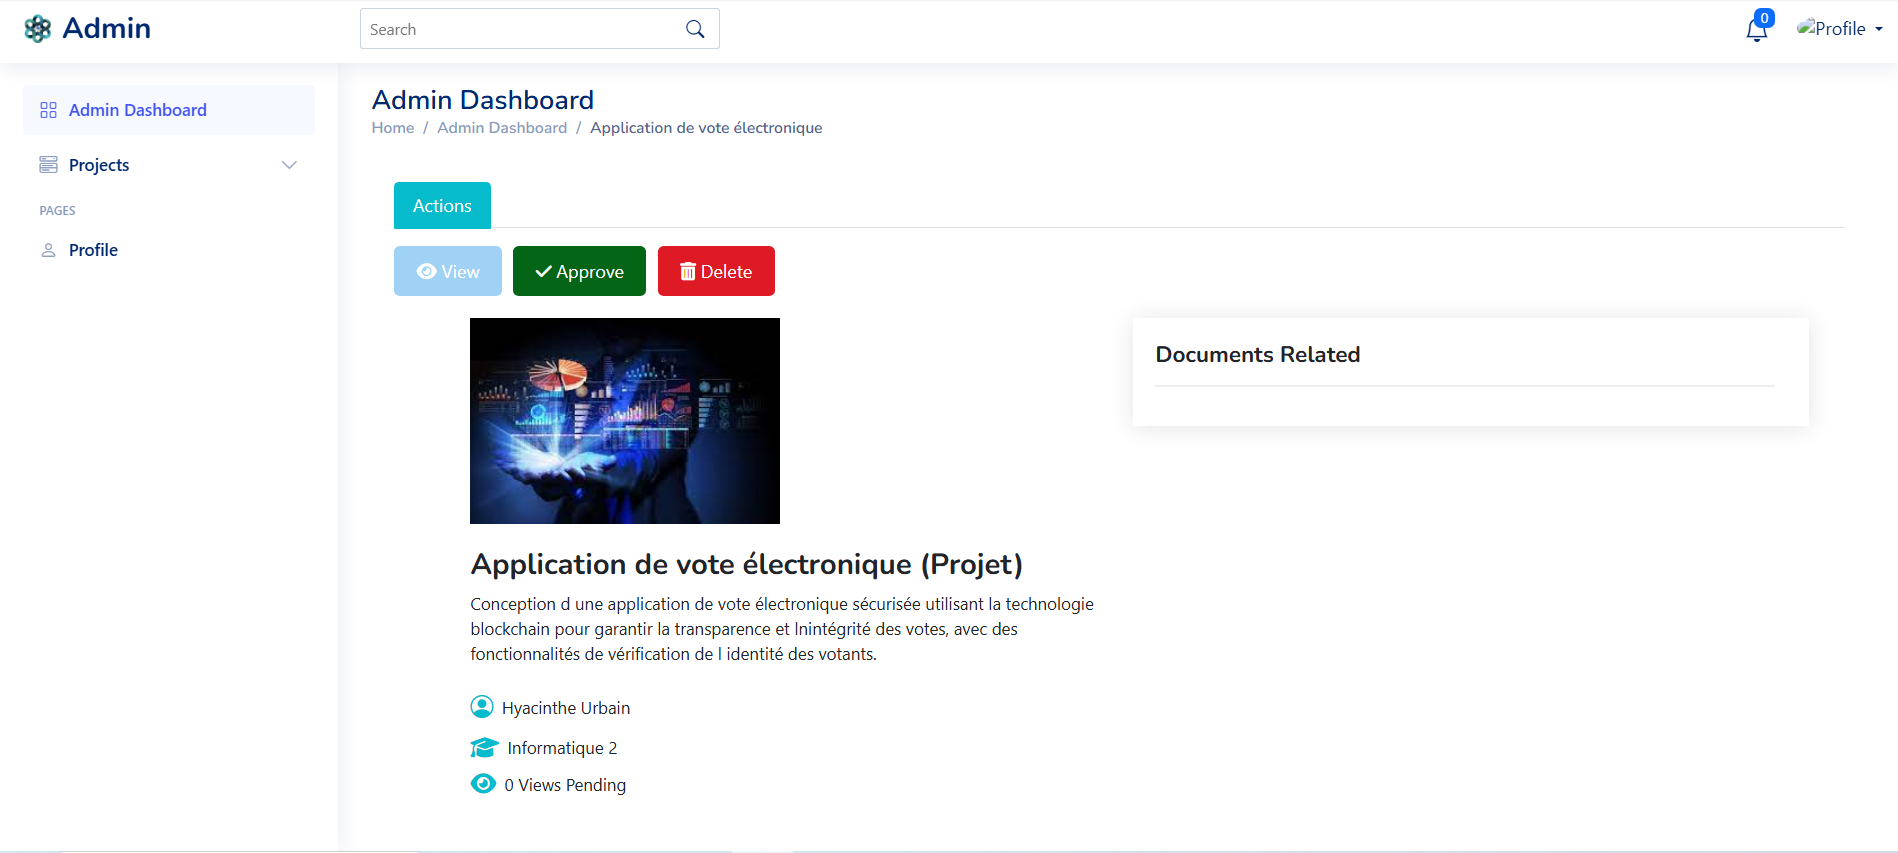
\includegraphics[width=\textwidth]{chemin/vers/image_gestion_statut.png}
\vspace{0.5cm}

\subsection{Organisation et Tri}

Le tableau des projets peut être trié selon différents critères : titre, auteur, statut, etc. Cette fonctionnalité optimise l’organisation et l’accès rapide aux données souhaitées.

% Illustration suggérée : Aperçu des options de tri dans le tableau des projets

\vspace{0.5cm}
\textit{Enfin, l’illustration suivante montre comment le tri dynamique est appliqué.}
% 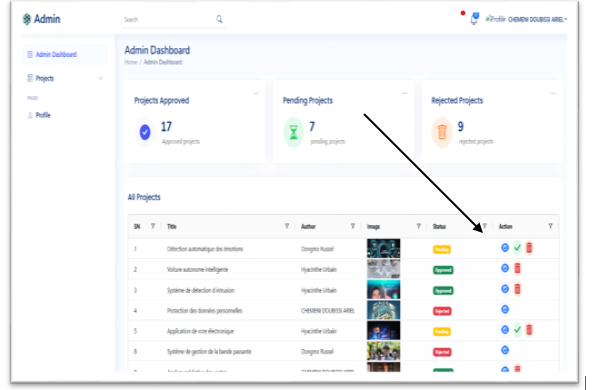
\includegraphics[width=\textwidth]{chemin/vers/image_tri_tableau.png}
\vspace{0.5cm}

\end{document}
